\begin{slide}{Syntax}
	\begin{itemize}
		\item{Syntax basiert auf Lochkarten}
	\end{itemize}
	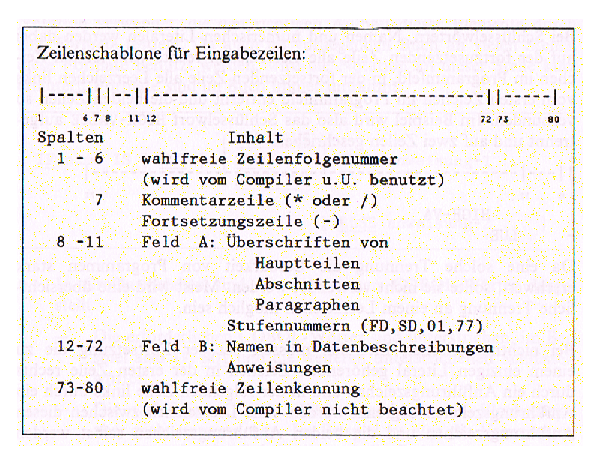
\includegraphics[scale=0.8]{syntax}\\
	Quelle: Einführung in die Programmiersprache COBOL
\end{slide}

\begin{slide}{Programmaufbau}
	\begin{itemize}
		\item{4 Hauptteile:
			\begin{itemize}
				\item{Erkennungsteil - \texttt{IDENTIFICATION DIVISION} }
				\item{Maschinenteil - \texttt{ENVIRONMENT DIVISION}}
				\item{Datenteil - \texttt{DATA DIVISION}}
				\item{Verarbeitungsteil - \texttt{PROCEDURE DIVISION}}
			\end{itemize}		
		}
	\end{itemize}
\end{slide}

\begin{slide}{Erkennungsteil}
	\begin{itemize}
		\item{Angabe von folgenden Informationen:
			\begin{itemize}
				\item{\texttt{PROGRAM-ID} - Programmname
					\begin{itemize}
						\item{Angabe an erster Stelle Pflicht}
						\item{Format des Namens divergiert bei Compilern}
					\end{itemize}				
				}
				\item{Nicht zwingend nötig:
				\begin{itemize}
					\item{\texttt{AUTHOR} - Name des Programmautors}
					\item{\texttt{INSTALLATION} - Name der Einrichtung}
					\item{\texttt{DATE-WRITTEN} - Datum der Programmerstellung}
					\item{\texttt{SECURITY} - Angabe von Sicherheitsvermerken}
				\end{itemize}
				}
			\end{itemize}		
		}
	\end{itemize}
\end{slide}

\begin{slide}{Maschinenteil}
	\begin{itemize}
		\item{Nicht zwingend notwendig}
		\item{\texttt{CONFIGURATION SECTION} - Konfigurations-Kapitel:
			\begin{itemize}
				\item{\texttt{SOURCE-COMPUTER} - Bezeichnung des Computers, auf dem kompiliert wird}
				\item{\texttt{OBJECT-COMPUTER} - Bezeichnung des Computers, auf dem ausgeführt wird}
				\item{\texttt{SPECIAL-NAMES} - verschiedene Anpassungen bspw.:
					\begin{itemize}
						\item{\texttt{DECIMAL-POINT IS COMMA.}}
					\end{itemize}				
				}
			\end{itemize}		
		}
		\item{\texttt{INPUT-OUTPUT SECTION} - Regelung der Ein- und Ausgabe:
			\begin{itemize}
				\item{\texttt{FILE-CONTROL} - Zuweisung von Geräten zu Dateien
					\begin{itemize}
						\item{\texttt{SELECT} dateiname \texttt{ASSIGN TO} systemname.}
					\end{itemize}				
				}
			\end{itemize}		
		}
	\end{itemize}
\end{slide}

\begin{slide}{Datenteil}
	\begin{itemize}
		\item{Nicht zwingend notwendig}
		\item{Unterteilt in drei Kapitel:
			\begin{itemize}
				\item{\texttt{FILE SECTION} - Deklaration interner Dateien}
				\item{\texttt{WORKING-STORAGE SECTION} - Verwaltung des Arbeitsspeichers
					\begin{itemize}
						\item{\texttt{sn var PICTURE IS datentyp VALUE IS wert.}}
					\end{itemize}				
				}
				\item{\texttt{LINKAGE SECTION} - Verbindungskapitel}
			\end{itemize}		
		}
	\end{itemize}
\end{slide}


\begin{slide}{Verarbeitungsteil}
	\begin{itemize}
		\item{Notwendig}
		\item{Enthält die Prozeduren}
	\end{itemize}
\end{slide}
